
\section{Understanding the domain} \label{sec:domain-overview}

The purpose of memory profilers is capturing information regarding how applications use memory.
To write profilers, a clear understanding about their nature is required.
Informally, the term \textit{memory profiling} refers to any kind of \textbf{process to collect} some \textbf{data about memory usage}.
In an object-oriented runtime environment, such data may be as simple as the number of objects of a specific class, but it may also be as complex as the list of possible memory leak's sources.
Some other examples include computing the number of objects reachable from a specific class object; finding out if there is an instance of class $A$ which is referencing an object of class $B$; and computing, for each \textit{String}, its length and the number of objects that make direct reference to the \textit{string}.
The data collected by a profiler may have an arbitrary complexity; it may be a simple natural number, a boolean value, a list of values, or a composed value.
For instance, an integer value is required to describe one of the aforementioned examples, the number of objects reachable from a specific class object.
In the same way, a pair $\langle l,r \rangle$, where both $l$ and $r$ are integers, is required to store the result of determining for a \textit{string}, its length and the number of objects referencing it.
%The data collected by a profiler may have an arbitrary complexity

%The rest of this section introduces the vocabulary we use in the domain of memory profilers.

Formally, we use a set of concepts to properly define our understanding of the term profiler, and how we address their construction in this chapter.
The following concepts are used int the rest of the chapter:

\begin{description}
\item[Object] is an atomic entity that consumes memory to store the value of its attributes.
When we say \textit{object} we mean as in \gls{OOP}.
The operations that we can perform on these objects are nevertheless restricted to accessing attributes, obtaining the amount of memory used to represent an object, and accessing meta-data such as the class name.
Reusing the concept is ``natural'' since we are targeting MRTEs, which often support the object-oriented paradigm.

\item[Memory Heap] As mentioned, this is the region of memory used to store dynamically allocated \textit{objects} that are connected through references -- forming a directed graph.
It is also the universe $\mathbb{U}$ of objects.

\item[Structure] is a subset of \textit{objects} in the \textit{memory heap}.
The objects in a structure don't need to be directly related by references; instead, they can be arbitrarily composed.
For instance, the smallest non-empty \textit{structure} we can consider, is a structure containing a single object.
Only one property is required in properly formed structures;  $S_1 \bigcap S_2 = \emptyset$ for any pair of structures $S_1$ and $S_2$, which means that they are disjoint sets.

\item[Memory Profile] is a value that can be computed using information from the \textit{objects} (and their references) included in a \textit{structure}.
An example of useful value is the total size of a structure, which can be easily calculated using the function $\textit{total\_size}\left(S\right) = \sum_{o \in S} {sizeof(o)}$.
A common pattern of use is to identify many \textit{structures} in the heap, and then to compute a value -- not necessarily the same -- for each structure.

\item[Memory Profiling] consists in identifying \textit{structures}, and computing some values associated to these structures. 

\item[Structure types] provide a mean to identify several structures using a single description.
In other words, since the heap can be partitioned in many structures, it is hard to manually enumerate them.
We need a procedural way to describe what are the structures we are considering (i.e., their membership functions), and what data we want to compute on each one of them; \textit{structure types} provide such facilities.

%Structure types parametrizado 
In particular, they provide (i) functions to evaluate whether an object is member of a \textit{structure}, (ii) ways to define the values corresponding to the \textit{memory profile} of a \textit{structure}, and (iii) factories to identify all \textit{structures} in the \textit{heap}.

\end{description}

%\extracomment{TODO}{Add example of structures in a graph, all connected to the fact that roots are in threads}

As mentioned, the objects in the heap form a directed graph; a profiler must iterate over such objects to identify whether they belong to a structure.
The following examples show what kind of operations must be executed during graph exploration.

\paragraph{Objects reachable from a specific class object}

Figure~\ref{fig:reachable-from-class-object} depicts a diagram of objects.
Suppose we want a profiler to compute the number of objects that can be reached from the object of class \textit{java.lang.Class} whose \textit{classname} is ``Client'' (see Figure~\ref{fig:reachable-from-class-object}).
Informally, this profiler must execute three steps to calculate the desired data.
First, it iterates over the objects to find all the instances of class \textit{java.lang.Class}.
These objects are then explored to get the value of attribute \textit{classname}, and see if it is equal to ``Client''; in this way we can locate the instance of interest.
Finally, the profiler traverses the graph (as in Depth First Search) using the node found in the previous step as root, and counting the number of traversed nodes.
In Figure~\ref{fig:reachable-from-class-object} the objects to count are highlighted.

\begin{figure}[!ht]
\centering
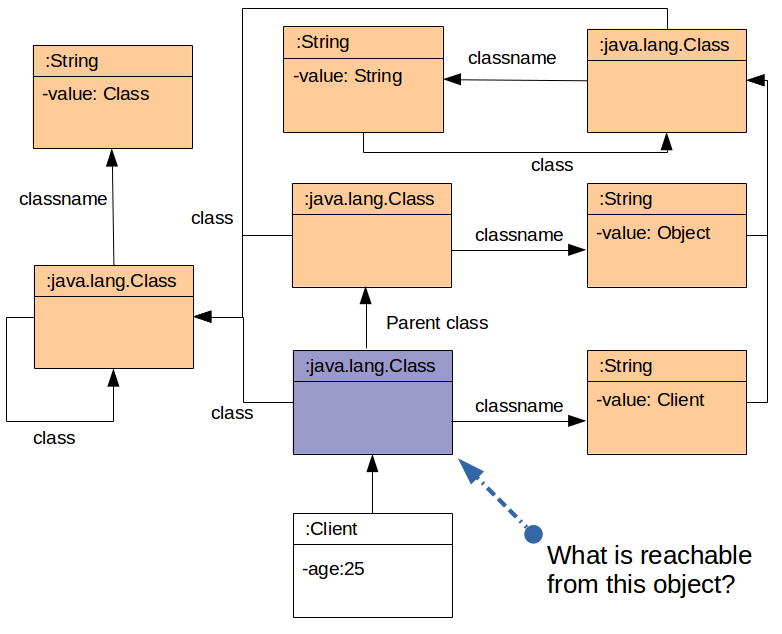
\includegraphics[scale=0.5]{./chapter6/fig/example1.png}
\caption{Objects reachable from the Client class. Observe that only one object is not reachable.}\label{fig:reachable-from-class-object}
\end{figure}

The aforementioned informal steps show what a profiler should be capable of doing:

\begin{itemize}
\item \textbf{Accessing meta-data of objects} such as the class of an object (\textit{java.lang.Class}), and the size of an object. 

\item \textbf{Accessing the value of attributes} is also helpful to filter out elements of the heap.

\item \textbf{Traversing references} is necessary because often some objects belong to a structure only because they are referenced by an object that is already a member.
\end{itemize}

To summarize, a function to determine whether an object is member of an structure may use: properties of the object itself, and properties about its relationships.

%\paragraph{Is there an instance of A making reference to an object of type B?}

%\paragraph{Length of each string, and number of objects referencing each string}

\paragraph{Nodes in each simply linked list}

In a second example, we want to calculate how many nodes has each simply linked list in the heap.
Figure~\ref{fig:simple_snapshot} shows a heap with two simply linked list and one double linked list.
The first list has three nodes while the second one has four; these are the values we want to obtain.

%Mostrar como hay patrones similares que se pueden detectar muchas estructuras
%Que entonces lo que se hace es describir el tipo de estructura con un paramtero adicional.

\begin{figure}[!ht]
\centering
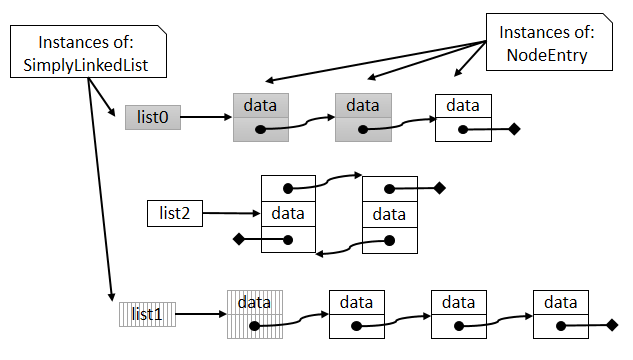
\includegraphics[width=0.65\linewidth]{chapter6/fig/lists}
\caption{Memory snapshot with three linked lists}
\label{fig:simple_snapshot}
\end{figure}


Informally, to compute such data a profiler must traverse the heap, checks whether an object's class is \textit{NodeEntry} (membership function), and increases a counter every time an instance is found (function to compute memory profile).
Unfortunately, these two steps are insufficient to correctly compute the fact that there exist two lists.
Indeed,  instead of the two values 3 and 4, a single value -- seven -- is obtained when this procedure is used.
The problem is that we have two structures instead of one, but using the aforementioned membership function it is impossible to know of which structure an instance of \textit{NodeEntry} is member of.
In other words, we need additional information to distinguish the two structures.

A method to solve this particular problem is to use the following recursive membership function: an object is member of a structure $S$ if it is an instance of \textit{NodeEntry} and it is being referenced by a member of $S$.
For the non-recursive case, we can see how each simply linked list starts with an instance of \textit{SimplyLinkedList}.
This is easily represented with a parametrized and recursive membership function:

\begin{equation} \label{eq:simply-list}
	f_{head}\left(O\right) = 
	\begin{cases}
		head = O & \quad O \; is \; \operatorname{SimplyLinkedList} \\
		\exists {x \in \operatorname{Objects}}, \quad x \operatorname{references} o \wedge f_{head}\left(x\right) & \quad O \; is \; \operatorname{NodeEntry} \\
		\operatorname{false} & \quad \operatorname{otherwise} \\
	\end{cases}
\end{equation}

The parameter $\textit{head}$ represents the structure of interest, and it is an instance of \textit{SimplyLinkedList}.
In this example, we have two functions, in which only the parameter varies, because there are two instances of class \textit{SimplyLinkedList}.
Similarly, we need two counters to store the number of nodes while we are traversing the graph of objects; once again, they (and the function to compute their values) are parametrized by the $head$ of the list.
Figure~\ref{fig:simple_snapshot} depicts a snapshot in time of the heap while it is being explored;
the shaded nodes are those that were already explored.

This example shows that in defining memory profilers, we often need the capacity for:

\begin{itemize}
\item Using the same functions for many structures, varying only some parameters. This is necessary for both membership functions and to compute the memory profile.

\item Identifying structures in the heap by using a parameter. For instance, in this example, we know that there are two structures because there are two instances of class \textit{SimplyLinkedList}.
\end{itemize}

To summarize, we are frequently interested in calculating values for many structures that have the same ``characteristics''; this is what we call \textit{structure type}.
To identify such structures we use a \textit{parameter}; the process of associating a particular parameter value to a structure type is done by a \textit{factory of structures}. 

\section{Metalanguage to define custom memory profilers}\label{sec:approach}

%In this chapter, we propose a tool to create custom memory profilers for MRTEs.
%We are interested on easing the task of defining new profilers without sacrificing their performance regarding CPU consumption.
%This section presents our approach, a metalanguage to define custom memory profilers in MRTEs.
%First, we present a global view of how our approach is used to support resource-aware programming, and how it integrates in a production environments (see Section~\ref{sec:dsl-global-architecture}).

%Keeping the profiler's overhead as low as possible is of utmost importance for us because lightweight profilers can be use both during the development phase and during the application execution in a production environment.
%To reach this goal, we propose a Domain Specific Language (DSL) and its code generator which aims at describing and generating efficient online memory profilers. 

%We next present the syntax, semantics and usage examples of our domain-specific language.


%\subsection{Global Architecture}\label{sec:dsl-global-architecture}

A global view of our approach is shown in Figure~\ref{fig:dsl-global-view}.
% the figure depicts how to and how it is integrated in production environments, are shown in .
Since our goal is to support resource-aware programming, in this architecture, an application is able to collect data on its own memory consumption.
To provide this feature, we add a layer (data collection layer) to MRTEs to take care of: 

\begin{itemize}
\item Providing a set of interfaces for collecting meta-data of objects in the heap, iterating over such objects, and reading the value of their fields.
These interfaces are used by memory profilers.

\item Providing a set of interface for accessing memory profilers from the applications.
In other words, an application may trigger the execution of a memory profiler, and it should be able to analyze the values computed by the profiler.

\item Supporting dynamic loading of memory profilers.
This is helpful in production environments for loading new dynamic analysis tools without having to stop the MRTE.
\end{itemize}

\begin{figure}[!ht]
\centering
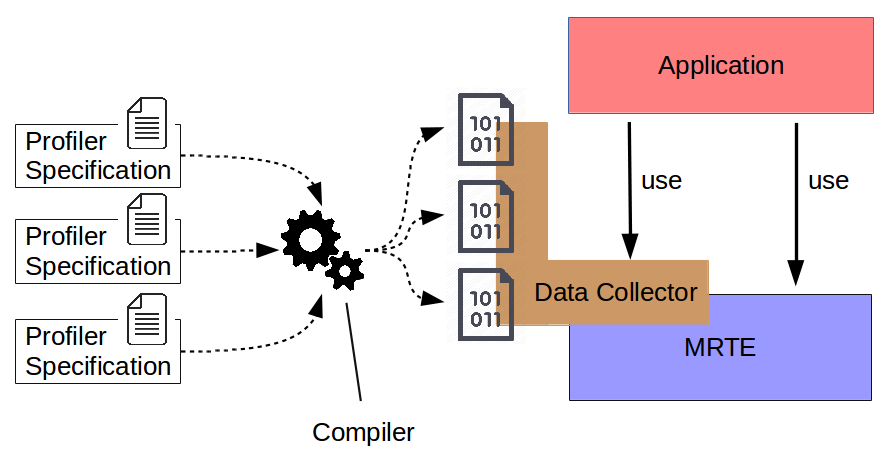
\includegraphics[scale=0.4]{./chapter6/fig/global-view.png}
\caption{Global view of the system. In this case, three memory profilers are defined.}\label{fig:dsl-global-view}
\end{figure}

In Figure~\ref{fig:dsl-global-view}, three memory profilers are plugged to the data collection layer.
The exact mechanism to collect raw data from the MRTE, as well as the mechanisms to dynamically load profilers, are platform specific.

A memory profiler can be handcrafted and plugged in this architecture; this is, nevertheless, error-prone.
Instead, we favor a generative approach where profilers are written using a metalanguage that hides low-level details.
A compiler is then used to transform such definitions into a binary form that can be executed in the runtime environment.
This compiler is also in charge of providing interoperability between the data format provided by low-level facilities of the MRTE, and the high-level data format expected by applications running on top of such execution environments. 

In the rest of this section we describe the elements of this architecture.
First, the abstract syntax of this metalanguage is discussed; we present it using a meta-model with its main concepts as well as some snips of code, written in a concrete syntax, to ease the presentation (see Subsection~\ref{sec:abstract-syntax}).
This concrete syntax is then introduced in Subsection~\ref{sec:concrete-syntax}, followed by 
\ifoperationalSemanticsOn
both the operational and
\else
the
\fi
translational semantic of the language (see 
\ifoperationalSemanticsOn
Subsections~\ref{sec:operational-semantic} and
\else
Subsection
\fi
\ref{sec:translational-semantic}).
Finally, in~\ref{sec:dsl-usage-examples} we present some examples of how to use the language.


\subsection{Abstract Syntax}\label{sec:abstract-syntax}

The meta-model shown in Figure~\ref{fig:as} describes the abstract syntax of our language.
The main concept of this meta-model is a \textit{CustomProfiler} which is composed of \textit{UserDefined} types and a \textit{StructureFactory}.
This means that a developer must focus on declaring the types to store information about memory usage, and defining the what are the \textit{structures} of interest by mean of \textit{factories}.

The concepts related to \textit{UserDefined} types are depicted on the left part of the metamodel, while the right part describes the \textit{StructureFactory} which represents both the set of  structures to identify and the value to compute on these structures.

\begin{figure*}
\centering
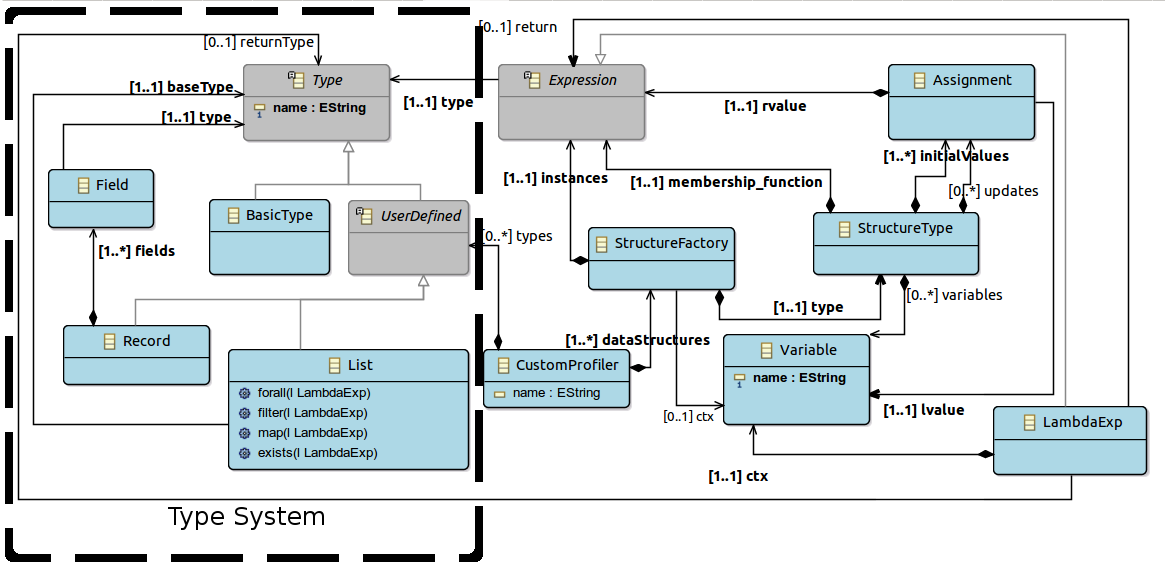
\includegraphics[width=0.93\linewidth]{chapter6/fig/AS}
\caption{Custom profiler Meta-model}
\label{fig:as}
\end{figure*}

\subsubsection*{User-defined types}
The language support three basic types -- \textit{Integer}, \textit{String} and \textit{Boolean}.
They are not shown in the meta-model for the sake of clarity, and because these types behave mostly as in any other language.

In addition, the language supports the declaration of both \textit{Records} and \textit{Lists}.
A \textit{record} is a compound type that contains \textit{fields} to hold values of previously defined types.
On the contrary,  all the members of a list must be of the same type; hence, a \textit{list} refers to a \textit{base type}.
In a profiler, \textit{UserDefined} types can be composed in any desired way as long as a single property is respected -- no recursive types are allowed.
We can formalize such a constrain using OCL (Object Constraint Language~\footnote{\url{http://www.omg.org/spec/OCL/}}):

\begin{lstlisting}[escapeinside={(*}{*)},
label=fig:membership,
language=OCL1
]
context Record inv: 
   not fields->oclAsSet()->closure(t)->exists(t | t = self)

context List inv:
   not baseType->oclAsSet()->closure(t)->exists(t | t = self)
\end{lstlisting} 

We enforce this constrain for two reasons. First, it simplify the type system, and second because it is a way to know that no data structure other than the built-in will be used to store a \textit{list}.
In this way, we can guarantee the performance of operations on lists.  
The \textit{List} type provides operations to manipulate list values.
In general, these operations correspond to the set of \textit{standard} operations of any implementation of the list data type in functional languages.
Table~\ref{tab:operations-on-lists} shows the name of these operations as well as their signature.

\begin{table}[!ht]
\centering
\begin{tabular}{r p{0.5cm} l}
\hline
\hline filter & & ('a $\to$ boolean) $\to$ 'a list $\to$ 'a list \\ 
forall & & ('a $\to$ boolean) $\to$ 'a list $\to$ boolean \\ 
exists & & ('a $\to$ boolean) $\to$ 'a list $\to$ boolean \\ 
%\hline foreach & & ('a $\to$ void) $\to$ 'a list $\to$ void\\ 
map & & ('a $\to$ 'b) $\to$ 'a list $\to$ 'b list \\ 
add & & 'a $\to$ 'a list $\to$ 'a list \\ 
first & & 'a list $\to$ 'a \\
\hline 
\end{tabular} 
\caption{Operations on lists.} \label{tab:operations-on-lists}
\end{table} 

In Listing~\ref{lst:defining-data}, a data structure to store information about a heap structure is declared.
First, a list (tableOf) of string is declared, it may be used to store the class name of objects.
Afterwards, a \textit{record} with two integer fields and a list field is declared in line 2.
This record may be used to hold values during profiling.

\begin{lstlisting}[escapeinside={(*}{*)}, 
label={lst:defining-data}, caption={Declaring types to store the number of object in a structure, its total size, and the class name of each object.}, language=DSL2
]
names: tableOf string
data: struct {
	total_size: int
	nr_objects: int
	classnames : names
}
\end{lstlisting}

\subsubsection*{Defining structures to profile}
Defining \textit{StructureFactories} is at the core of writing a custom profiler.
A \textit{StructureFactory} contains an \textit{Expression} through the \textit{instances} relationship, which indicates a pattern to identify structures in the memory heap.
Notice that a single instance of \textit{StructureFactory} identifies many structures in memory; thus, the \textit{Expression} is a list -- a new structure must be instantiated for each element of the list.
%Forcing the \textit{Expression} to be a \textit{List} can be easily formalized using OCL:

%\begin{lstlisting}[escapeinside={(*}{*)}, label=fig:instances, language=OCL1]
%context StructureFactory inv: instances.type.oclIsTypeOf(List)
%\end{lstlisting}

Listing~\ref{lst:defining-header} shows a snip of code that defines a structure for each \textit{SimplyLinkedList} in the heap.
This is useful to solve one of the example we mentioned in Section~\ref{sec:domain-overview}.
Note that `$e$' is the \textit{value} used to parametrize the structures.
In this case, `$e$' will take the values in the list defined after `$:$'; such a list is composed by instances of class \textit{SimplyLinkedList}.
In this example, we use the operation \textit{filter} on a built-in list -- \textit{objects}.
The actual parameter for \textit{filter} is a lambda expression that only return true if its parameter is an instance of the expected class. 

\begin{lstlisting}[escapeinside={(*}{*)}, 
label={lst:defining-header}, caption={Defining a factory that instantiates a structure for each instance of the class SimplyLinkedList that it can find in the heap.}, language=DSL2
]
create structure foreach e: objects.filter([
		o | 
		  ret o is SimplyLinkedList
		]) using
\end{lstlisting}

Defining a new \textit{StructureFactory} implies defining a \textit{StructureType}.
This concept describes the mechanism used to identify a structure and compute some values.
A \textit{StructureType} is composed of \textit{Assignments} that are used as \textit{initialValues} for each \textit{Variable} holding a value of the structure -- similar to a constructor in \glslink{OOP}{OOP}.
In addition, a \textit{StructureType} contains a boolean \textit{expression} which is the \textit{membership function} used to decide whether an object is member of the structure.
Finally, it also contains \textit{assignments} to update the value of each \textit{variable} every time an object is added to the structure.
%These \textit{assignments} are used to compute the actual value of the memory profile.
The major constraint regarding these \textit{updates} is that they must refer to already initialized \textit{variables}, and the new assigned values must match the previous types.
We formalize such a constrain using OCL:

\begin{lstlisting}[escapeinside={(*}{*)}, label=fig:lvalue, language=OCL1]
context StructureType inv:  updates->forAll(a: Assignament | 
    self.initialValues->exists(aa : Assignament | 
       aa.lvalue = a.lvalue and aa.rvalue.type = a.rvalue.type
     ))
\end{lstlisting}


In Listing~\ref{lst:listLengt}, we show how to compute the length of each \textit{SimplyLinkedList} in the memory snapshot depicted in Figure~\ref{fig:simple_snapshot}.
We use the fact that each \textit{NodeEntry} points to the next element in the list.
Since we only want to count the number of nodes in each list, we simply define an \textit{integer} variable in the structure type -- `$n$'; in line 7, this variable is updated every time an object is added to the structure.
The variable `$e$' is used to parametrize the structure; observe how, in line 3, a list of members of the structure is initialized (`$e$' is its only member).
This line corresponds to defining the non-recursive case of the membership function.
Line 1 was already discussed, it is just worth highlighting that only two structures will be built because there are two simply linked lists in the memory snapshot.
The first member of these structures are in one case \textit{list0}, and \textit{list1} in the other case.
 

\begin{lstlisting}[escapeinside={(*}{*)}, 
label={lst:listLengt}, caption={Calculating the length of each simply linked list.}, language=DSL2
]
create structure foreach e:objects.filter([o| ret o is SimplyLinkedList]) using
  constructor
    initialObjects = #[e] // a list literal with one element: e
    n = 0
  membership (this is NodeEntry) and (referrer in this_structure)
  updates 
    n = n + 1
\end{lstlisting}

The recursive case of the membership function is in line 5.
It resembles the definition in function \ref{eq:simply-list}; there are however differences that are due to the evaluation semantic of our language.
Although the semantic is discussed hereafter, we can understand the definition by simply knowing that it is evaluated for every edge of the directed graph.
Before the evaluation, three variable are created: \textbf{this}, \textbf{referrer}, and \textbf{this\_structure}; they are, respectively, the target of the edge, the source, and a structure.
When we evaluated the membership function we are simply checking whether \textbf{this} is a member of \textbf{this\_structure}, and we are passing additional information to support the definition of recursive functions.


%Once a new structure is created, the \textit{Assignments} are executed to assign the initial value of each \textit{Variable}.

\subsubsection*{Expressions and Types}


Nevertheless, there is a built-in variable in each \textit{StructureType} that is only accessible during initialization.
Its type is predetermined as part of the language specification.
We force the use of the proper type using OCL:

\begin{lstlisting}[escapeinside={(*}{*)}, label=fig:instances, language=OCL1]
context StructureType inv:  initialValues->exists(a: Assignment | 
     a.lvalue.name = 'initialObjects' and a.rvalue.type.oclIsTypeOf(List)
   ) 
\end{lstlisting}


For the sake of readability, Figure~\ref{fig:as} only shows a few concepts related to expressions.
In addition to \textit{arithmetic}, \textit{boolean} and \textit{literals} for basic types, the language includes lambda expressions, literal for records and lists.

Observe that \textit{variables} do not refer to a \textit{Type}; indeed, the language is  strongly typed, and the \textit{type} of each user-defined variable is inferred from its initial value.
To support type-inference, the type of each expression is clearly defined.

Built-in rvalues, which are nothing but expressions initialized by the runtime within a specific scope, and their types are also defined.
There are two types of built-in rvalues -- platform independent and dependent.
Among the firsts, we have the list of  \textit{\textbf{objects}}, the list of \textit{loaded classes} (\textbf{classes}), a reference to the \textit{current data structure} (\textbf{this\_structure}), and a reference to the \textit{current object} (\textbf{this}).
Target dependent \textit{rvalues} include the list of \textit{threads} (\textbf{threads}) and the type of reference (\textbf{reference\_kind}).

Built-in rvalues are only valid in specific contexts.
For instance, \textbf{this}, \textbf{referrer}, \textbf{this\_structure}, and \textbf{reference\_kind}, exist either during the evaluation of the membership function or when the variables are being updated.
On the contrary, the values \textbf{objects}, \textbf{classes}, and \textbf{threads}, are valid only during the creation of structures and their initialization.
Since building rvalues of type list is costly in terms of performance overhead, we decide avoiding their use in membership functions and updates. 
 
%The precise meaning of these \textit{rvalues} are discussed in Subsections~\ref{sec:translational-semantic}, and~\ref{sec:implementation}.

%The valid scope of this rvalue is in both the definition of the set of structures and the computation of the initial values.

%There are four built-in rvalues during the evaluation of the function as well as during the update of the variables.
%First, the value named \textit{this} is the current visited object. 
%The value \textit{this\_structure} identifies the structure.
%As our runtime profiler will traverse the graph of in memory objects following references between objects, the object through which we have reached the \textit{this} object is known as \textit{referrer}.
%The last value, which is target dependent, is the kind of reference.

\subsection{Concrete Syntax}\label{sec:concrete-syntax}

A textual concrete syntax has been defined for our language; using it, a domain expert can define a custom memory profiler using a text editor.
A grammar for this textual representation is depicted in Figure~\ref{fig:dsl-grammar}.
Notice how the rules for expressions make such a grammar ambiguous; we decide to use this form to ease the presentation.
However, a complete LL(*) grammar~\cite{Parr:2011:LFA:1993498.1993548} can be found in Appendix~\ref{anx:grammar}.
One interesting aspect of this concrete language is its relative verbosity.
For instance, it uses very explicit keywords such as ``create structure foreach'', ``constructor'', and ``membership''.


%\setlength{\grammarparsep}{20pt plus 1pt minus 1pt}
{
\scriptsize
\begin{figure}[!ht]
\begin{mdframed}[outermargin=0.2cm, innermargin=0.5cm]

\newcommand{\grule}[1]{\hfill{\scriptsize (#1)}}
\setlength{\grammarindent}{4em}
\begin{grammar}

<program> ::=  `name' <string-literal> <types> <structures> \grule{1}

<types> ::= <type> <types> | <empty> \grule{2, 3}

<type> ::= <id> `:' `tableOf' <id> | <id> `:' `struct' `{' <fields> `}' \grule{4, 5}

<fields> ::= <id> `:' <id> <fields> | <id> `:' <id> \grule{6, 7}

<structures> ::= <factory> <structures> | <factory> \grule{8, 9}

<factory> ::= `create structure foreach' <id>`:'<e> `using' <body> \grule{10}

<body> ::= `constructor' <s> `membership' <expr> `updates' <s> \grule{11}

<s> ::= <a> <s> | <empty> \grule{12}

<a> ::= <id> `=' <e>  \grule{13} 

<e> ::= <e> <op> <e> | <u-op> <e> | <e> `in' <id> | <e> `is' <id> \grule{14, 15, 16, 17}
\alt <e> `.' <id> `(' <expr-list> `)' | <e> `.' <id> \grule{18, 20}
\alt `#' <l-type> `[' <expr-list> `]' | `struct' <id> `{' <expr-list> `}' \grule{21, 22}
\alt <int-literal> | <string-literal> | <bool-literal> \grule{23, 24, 25}
\alt <id> | `(' <e> `)' | `[' <id> `|' <s> `ret' <e> `]' \grule{26, 27}
\alt <e> `?' <e> `:' <e>

<expr-list> ::= <e> `,' <expr-list> | <empty>  \grule{28}

<l-type> ::= <id> | <empty>

<op> ::= `+' | `*' | `-' | `/' | `and' | `or' | `>' | `<' | `>=' | `<=' | `==' | `!='

<u-op> ::= `-' | `not'

\end{grammar}
\end{mdframed}
\caption{Concrete grammar of the language. For the sake of clarity, we are using an ambiguous grammar to describe the expression language.} \label{fig:dsl-grammar}
\end{figure}
}


An interesting aspect of this grammar is how \textbf{list} and \textbf{struct} values are defined.
In particular, they can be created from non-constant values in the right hand of the evaluation.
For instance, in Listing~\ref{fig:declaring-structures}, three values are created; line 1 instantiates a list of integers with two elements, line 2 defines a value of type \textit{Point}, and line 3 creates an empty list of \textit{strings} that is immediately populated with one element.
Notice that line three requires writing the type of the list because it is not possible, in general, to infer the list type. 

\begin{lstlisting}[escapeinside={(*}{*)}, 
label={fig:declaring-structures}, caption={Creating list and struct values.}, language=DSL2
]
l = #[ 4, n + 12]
s = struct Point { x , 14 }
m = #String[].add("first element")
\end{lstlisting}


%Observe the usage of a built-in \textit{rvalue} named \textit{objects} which contains all the objects in memory.
%The valid scope of this rvalue is in both the definition of the set of structures and the computation of the initial values.
%Thereafter, lines 2-4 specify the initial values.
%Line 3 in particular initializes the set of objects included in the structure.
%Notice the usage of a list literal to include the object referenced by \textit{e}.
%In the initialization scope, the rvalue \textit{e} is equal to one of the element within the list of structures - either \textit{list0} or \textit{list1}.

%In line 5 we define the membership function, which is used to determine if an object is part of the structure.
%There are four built-in rvalues during the evaluation of the function as well as during the update of the variables.
%First, the value named \textit{this} is the current visited object. 
%%The \textit{membership} boolean \textit{expression} aims at determining if this object is part of the \textit{structure} or not. 
%The value \textit{this\_structure} identifies the structure.
%As our runtime profiler will traverse the graph of in memory objects following references between objects, the object through which we have reached the \textit{this} object is known as \textit{referrer}.
%The last value, which is target dependent, is the kind of reference.
%Operator \textbf{is} checks if \textit{this} is an instance of class \textit{NodeEntry}.
%Likewise, operator \textbf{in} checks whether the \textit{referrer} is already a member of the structure.
%Finally, line 7 updates the length of the list when an object is detected as member of the structure.

\ifoperationalSemanticsOn
\subsection{Operational Semantics} \label{sec:operational-semantic}

\extracomment{TODO}{
\begin{enumerate}
\item Add notation
\item Fix the rule that calls a method with a lambda expression
\item Add the rule for the interpretation of a program
\item Discuss the inference rules
\end{enumerate}
}

\begin{figure}
\begin{mdframed}[innermargin=0.3cm, outermargin=0.3cm]

{
\footnotesize

\begin{tabular}{rcl}
$Bool(1)$ and $Bool(0)$ & & \parbox{8cm}{Values  $true$ and $false$.}\\
& & \\
$ E $ & \parbox[t]{0.7cm}{} & \parbox{8cm}{Describes a mapping from \textit{identifiers} to \textit{locations}. We use $id \mapsto l$ to represent a member of the mapping} \\ 
& & \\
$ S $ & & \parbox[t]{8cm}{Describes a mapping from \textit{locations} to \textit{values}. Informally, it can be seen as the storage. We use $l \mapsto v$ to represent a member of the a mapping.} \\ 
& &  \\
$ C $ & & \parbox[t]{8cm}{Describes a mapping from \textit{values} to \textit{structures}. We use $v \mapsto s$ to represent a member of the mapping.} \\ 
& & \\
$\left[ k_1 \mapsto v_2, \dots, k_n \mapsto v_n \right]$ & & \parbox[t]{8cm}{Describes a mapping by enumerating its members.} \\ 
& & \\
$S\left[ v_i/k_i \right]$ & & \parbox[t]{8cm}{Describes a new mapping where $S\left[ v_i/k_i \right](k_j) = S(k_j)$ if $k_i \ne k_j $, $S\left[ v_i/k_i \right](k_j) = v_i$ otherwise. } \\
& &  \\
$M \overset{\operatorname{val\_of}}{\vdash} k \mapsto v$ & & \parbox[t]{8cm}{A set of auxiliary rules to compute the value $v$ that is associated to the key $k$ in the mapping $M$.} \\ 
& &  \\
$C \overset{\operatorname{contains}}{\vdash} v \mapsto s \Rightarrow r$ & & \parbox[t]{8cm}{A set of auxiliary rules to determine whether the value of $v$ is mapped to $s$ in $C$, which is always a mapping from  \textit{values} to \textit{structures}. $r$ is a boolean value. } \\
& &  \\
$\lVert E,S, id, e\rVert$ & & \parbox[t]{8cm}{Describe a closure, $E,S$ represents the state, $id$ is the identifier used as parameter of the closure, and $e$ is the expression to evaluate.} \\ 
& & \\
$T(a_1 \mapsto l_1, \dots, a_n \mapsto l_n)$ & & \parbox[t]{8cm}{A generic value in the language. $T$ is its type, and a mapping from attributes $a_i$ to their respective locations $l_i$. Sometime, we use $\mathbb{A}$ to represent the mapping. There are shorthands for special cases: $Bool(1)$, $Bool(0)$, $Int(n)$ which is the integer $n$, and $String(w)$ which is the string $w$. In addition, the value $table(l_1,\dots,l_n)$ denotes a table; in this case, $l_i$ is the location in storage of the \textit{i-th} element of the table. } \\ 
& & \\
$\langle T, P, a_1 \mapsto T_1, \dots, a_n \mapsto T_n \rangle$ & & \parbox[t]{8cm}{Describe a type with identifier $T$. The description contains the parent type $P$ (which has the same structure), and its attributes $a_i \mapsto T_i$. } \\
& & \\ 
$\overset{\operatorname{subtype}}{\vdash} S, P \Rightarrow r$ & & \parbox[t]{8cm}{A set of auxiliaries rules to determine whether type $S$ is a subtype of $P$. $r$ is a boolean value.} 
\end{tabular} 

}

\end{mdframed}
\caption{Notation used in the operational semantic}\label{fig:notation-for-operational-semantic}
\end{figure}

\renewcommand{\inference}[3][]{%
  \begin{array}[b]{@{}c@{}c@{}}
    \smash{\raisebox{-.5\normalbaselineskip}{{\scriptsize #1}}} & 
      \begin{array}[b]{l}
        #2
      \end{array} \\
      \cline{2-2}
    & \begin{array}[t]{c}
        #3
      \end{array}
  \end{array}
}

\mathlig{->}{\mapsto}
\mathlig{|-}{\vdash}
\mathlig{=>}{\Rightarrow}
\mathlig{"}{\;\;\;}

\mathligson

% classics
{
\footnotesize
\[
% true
\textnormal{{\scriptsize It(25):}}\; E, S\vdash\operatorname{true}\Rightarrow Bool(1),S
\quad\quad
% false
\textnormal{{\scriptsize It(25):}}\; E, S\vdash\operatorname{false}\Rightarrow Bool(0),S
\]

\[
% integers
\textnormal{{\scriptsize It(23):}}\; E, S\vdash\operatorname{Integer}\; N\Rightarrow Int(N),S
\quad\quad
% strings
\textnormal{{\scriptsize It(24):}}\; E, S\vdash\operatorname{String}\; w\Rightarrow String(w),S
\]

% lambda expressions
\[
\textnormal{{\scriptsize It(19):}}\; E, S\vdash \left[id \vert e \right] \Rightarrow \lVert E,S, id, e\rVert,S
\]

\[
% id
\inference[It(26):]{
E\overset{val\_of}{|-}id->l_{id} "" S\overset{val\_of}{|-}l_{id}->v
%v = S \; E \; id
}{E, S|-id=>v,S}
\quad\quad
% (e) 
\inference[It(27):]{
E, S|-e=>v,S_1
}
{E, S|-(e)=>v,S_1}
\]

\[
% unary operators
\inference[It(17b):]{
E, S|-e_0=>v_0,S_1
}{E, S|-\operatorname{op}e_0=>\operatorname{op}v_0,S_1}
\quad\quad
% binary operators
\inference[It(17a):]{
E, S|-e_0=>v_0,S_1 "" E, S_1|-e_1=>v_1,S_2
}{E, S|-e_0\operatorname{op}e_1=>v_0\operatorname{op}v_1,S_2}
\]

\[
% in operator
\inference[It(17c):]{
C, E, S|-e_0=>v_0,S_1 "" C \overset {contains} {|-} v_0->id =>v
%v = v_0->id \in C? Bool(1):Bool(0)
}{C, E, S|-e_0 \; in \; id=>v,S_1}
\quad\quad
\]

\[
% is operators
\inference[It(17d):]{
E, S|-e_0=>X(\mathbb{A}),S_1 "" \overset{subtype}{|-} X, T \Rightarrow v
}{E, S|-e_0\; \operatorname{is} \; T:v,S_1}
\]

\[
% assignment
\inference[It(16):]
{
E,S|-e_0=>v_0,S_1 "" E\overset{val\_of}{|-}id->l_{id}
%l_{id} = E(id) \\
%S_2 = 
}
{E, S|-id = e_0=>v_0, S_1[v_0/l_{id}]}
\quad\quad
% statements
\inference[It(14)]
{
E, S|-a=>v_a,S_1 "" E, S_1|-s=>v,S_2
}
{E, S|-a\;s=>v,S_2}
\]

\[
% struct literal
\inference[It(22):]
{
E,S|-e_1=>v_1,S_1 \\
\vdots \\
E,S_{n-1}|-e_n=>v_n,S_n \\
\operatorname{class}(T)=(a_1->T_1, \dots, a_n->T_n) \\  % take the fields of the object
l_i = \operatorname{newloc}(S_n) \; for \; i = 1 \dots n \\
v=T(a_1->l_1, \dots, a_n->l_n) \\ % assign locations to fields
S_f = S_n[v_1/l_1, \dots, v_n/l_n]
}
{E, S|-struct\;T\;\{ e_1, \ldots, e_n \}:v,S_f}
\quad\quad
% list literal
\inference[It(21):]
{
E,S|-e_1=>v_1,S_1 \\
\quad \vdots \\
E,S_{n-1}|-e_n=>v_n,S_n \\
l_i = \operatorname{newloc}(S_n) \; for \; i = 1 \dots n \\
v=\operatorname{table}(l_1, \dots, l_n) \\
S_f = S_n[v_1/l_1, \dots, v_n/l_n]
}
{E, S|-\#[e_1, \dots, e_n]:v,S_f}
\]

\[
% accessing field
\inference[It(20):]{
E,S|-e=>X(\mathbb{A}),S_f "" \mathbb{A} \overset{val\_of}{|-} \textit{id} -> l_{\textit{id}} "" S \overset{val\_of}{|-} l_{\textit{id}} -> v
%v0 = X(a_1->l_1, \dots, a_n->l_n) \\
%l_{id} = l_i \; where \; a_i = id \\
%v = S_1(l_{\textit{id}}) \\
}
{E,S|-e.\textit{id}=>v,S_f}
\]

\[
% calling method
\inference[It(18):]{
E,S|-e_0=>X(\mathbb{A}),S_0 \\
E,S_0|-e_1=>v_1,S_1 \\
""" \vdots \\
E,S_{n-1}|-e_n=>v_n,S_n \\
\operatorname{impl}(X,f) = (x_1, \dots, x_n, f_{body}) \\
l_{x_i} = \operatorname{newloc}(S_{n+1}) \; for \; i = 1 \dots n \\
\mathbb{A}[l_{x_1}/x_1, \dots, l_{x_n}/x_n],S_n[v_1/l_{x_1}, \dots, v_n/l_{x_n}]|-f_{body}:v,S_f
}
{E,S|-e_0.f(e_1, \dots, e_n):v,S_f}
\]

% graph
%
% 1 - recorrer

\[
\inference[It():]{
\mathbb{(V,E)} \overset{struct}{|-} \textit{sf}_1, \dots, \textit{sf}_k => \left[ \textit{st}_1, \dots, \textit{st}_m \right],C,E,S "" \mathbb{(V,E)},C,E,S\overset{fill}{|-} \left[ \textit{st}_1, \dots, \textit{st}_m \right] => \left[ \textit{st}_1, \dots, \textit{st}_m \right], S_1
}{
\mathbb{(V,E)}|- \textit{sf}_1, \dots, \textit{sf}_k => \left[ \textit{st}_1, \dots, \textit{st}_m \right], E, S
}
\]

}



\mathligsoff

\fi

\subsection{Translational Semantics}\label{sec:translational-semantic}

A profiler written in this language is compiled to produce a custom memory profiler for a specific target platform.
%An instance of our metamodel is compiled into a custom memory profiler.
For instance, in our reference implementation, the compiler produces a library written in \textit{C++}, which is in charge of collecting the desired information from the runtime environment.
The generated source code is a set of classes.
In particular, for each \textit{StructureType} in the model, the compiler generates a subclass of \textit{AbstractStructure},  which is shown below.
Every subclass contains attributes to store the variables used in the associated \textit{StructureType}.
In the listing below, the class \textit{Context} holds built-in rvalues such as \textbf{objects}, \textbf{this}, and \textbf{referrer}.
\begin{lstlisting}[language=C++, frame=L,
numbers=left,
numberstyle=\color{black}\scriptsize,xleftmargin=2\parindent]
class AbstractStructure {
public:
	virtual void initialize(const Context& ctx) = 0; // correspond to constructor
	virtual bool membership(const Context& ctx) = 0; // membership function
	virtual void update(const Context& ctx) = 0; // update variables
}
\end{lstlisting}

Listing~\ref{dsl-generated-c-linked-list} shows the code generated by the compiler for the simply linked lists example (see Listing~\ref{lst:listLengt}).
Notice the use of three functions provided by the runtime, \textit{markAsMembers}, \textit{isInstance}, and \textit{isMember}. 

\begin{lstlisting}[language=C++, frame=L,
numbers=left,
numberstyle=\color{black}\scriptsize,xleftmargin=2\parindent, label=dsl-generated-c-linked-list,
caption={To represent a structure type, we declare a subclass of AbstractStructure.}]
class SimplyLinkedListStructure1 : public AbstractStructure {
private:
	int n;
public:
	void initialize(const Context& ctx) {
		vector<DSL_Object> l;
		l.push_back(ctx.e);
		markAsMembers(l, ctx.this_structure); // part of the language runtime support
		n = 0;
	}
	bool membership(const Context& ctx) {
		bool b0 = isInstance(ctx.this, "NodeEntry"); // part of the language runtime support
		bool b1 &= isMember(ctx.referrer, ctx.this_structure); // part of the runtime support
		return b1;
	}
	void update(const Context& ctx) {
		n = n + 1;
	}
	static void createStructures(const Context& ctx, vector<DSL_Object>& instances) {
		vector<DSL_Object> r;
		auto f = [](DSL_Object o) { return isInstance(o, "SimplyLinkedList")};
		ctx.objects.filter(f, r); // add valid elements to r
		instances.insert(instances.end(),r.begin(),r.end()); 
	}
}
\end{lstlisting}

The last function, \textit{createStructures}, is used to identify structures of this type.
They are invoked by a template initialization routine that expects as generic parameter a subclass of 
\textit{AbstractStructure} -- \textit{T} in Listing~\ref{lst:init-routines}.
Formally, the signature and behavior of this routine are as follow:
\begin{lstlisting}[language=C++, frame=L,
numbers=left,
numberstyle=\color{black}\scriptsize,xleftmargin=2\parindent,
label=lst:init-routines, caption={Routine to initialize structures in the heap.}]
template <typename T> void
initializationRoutine(Context& ctx, std::vector<AbstractStructure*>& s){
  vector<DSL_Object> instances;
  T::createStructures(ctx, instances);
  for (DSL_Object obj : instances) {
    AbstractStructure* ns = new T();
    ctx.e = obj;
    ctx.this_structure = defineStructure(ns); // part of the runtime support
    ns->initialize(ctx);
    s.push_back(ns);
  }
}
\end{lstlisting}
An important concern during the transformation lays on efficiently mapping our concepts to \textit{C++} concepts.
Moreover, since each target platform provides facilities to get metadata regarding the objects in memory, using such facilities efficiently is especially important in order to reduce the performance overhead due to profiling.

The final profiler is built using both the generated code and a template algorithm.
The template is target dependent, but in general we use the underline target facilities to collect meta-data, access fields in certain steps, traverse the objects in memory and also to populate the built-in rvalues.
A simplified version of this algorithm is shown in Listing~\ref{lst:dsl-algorithm}.

\begin{lstlisting}[escapeinside={(*}{*)},
label=lst:template, language=AlgLang, frame=L,
numbers=left,
numberstyle=\color{black}\scriptsize, xleftmargin=2\parindent,
label=lst:dsl-algorithm, caption{Template algorithm to collect data with in a memory profiler.}]
values:
   structures: vector<AbstractStructureType*>
routine:
   foreach (StructureType ST)
	  create context
	  call initializationRoutine<ST>(context, structures)
   
   foreach (r: references among objects)
      if (r.target has no membership)
         create context // context.this = r.target
         S = structures.findfirst(s | s.membership(context))
         make context.this a member of S
         S.update(context)
   return structures 
\end{lstlisting}

There are two loops in the algorithm. 
The first loop is in charge of creating the set of structures the program is intended to collect information about.
The creation of a context in line 5 depends on the target platform.
It basically creates values such as the list of objects in memory or the list of loaded classes.
The second loop traverses all the references among objects in memory.
During each iteration, the algorithm finds the first structure for which the membership function is true.
Notice that we only select the first because for some memory accounting problems, it is too hard to define a membership functions that build disjoints structures~\cite{dsn/09/geoffray/ijvm,Attouchi:2014:MMM:2602458.2602467}.
Thereafter, the information for such a structure is updated.

%The complete execution of a program in our language is as follow. Subgraph instances are initialized using listing~\ref{onInitialization}.
%Afterward, all the references in the graph of objects are traversed running listing~\ref{lst:onNodeFoundData}.
%The output data for all subgraph instances has been collected after all the references are traversed once.

%Finally, in listings~\ref{lst:onNodeFound},~\ref{lst:onNodeFoundData} and~\ref{onInitialization} we use built-in properties that are defined by the user.
%These properties must have access to some data describing the content of the memory in order to successfully identify subgraphs and calculate output values.
%Such data is wrapped in what we call execution context.
%In our DSL there are two different execution contexts: \textit{global context} and \textit{local context}.
%The former includes built-in values such as: i) lists of \textit{objects}, \textit{threads}, \textit{classes}, etc. , and ii) a value called \textit{Entity} representing a subgraph instance.
%The latter only contains the object \textit{THIS} which is being visited, a label of the reference representing its type, \textit{REFERRER} which is the object referencing the visited and again the \textit{Entity} value.
%The \textit{global context} is available in listing~\ref{onInitialization} while the \textit{local context} is available in both listings~\ref{lst:onNodeFound} and~\ref{lst:onNodeFoundData}.

\subsection{Language Usage} \label{sec:dsl-usage-examples}

There are several possibilities for using our DSL in the various stage of an application lifecycle.
For instance, checking invariants of data structures, computing memory consumption of different software abstractions, and checking reachability properties.
Some of these uses may help to support resource-aware programming, others may be useful to support additional tasks in software development.
In this section, we discuss some examples to highlight possible uses of our language.
%These include checking: local data structure invariants, reachability properties, memory consumption properties and combinations of those.
%Below, we show some examples to highlight possible usage of our language. 
 
\paragraph{Example 1: Evaluating an assertion}
The first example shows how to assess the existence of a value satisfying a property, independently of which object contains it.
Specifically, we want to check whether exists an object with an attribute named ``data'' whose value is between \textit{3} and \textit{5}.
Since the answer we expect is a simple boolean value, this example can be seen as a form of assertion regarding the memory content.

We can write a memory profiler to compute this value.
A complete code to implement it is depicted in Listing~\ref{lst:dsl-example1}.
Since we want to compute a single boolean value that depends on all the objects in the heap, this profiler only needs to create one structure.
In the code, this is shown in line 1, where the list of instances has one element.
Notice that we use the string value ``whole-jvm'', this has been arbitrarily chosen, any value is acceptable in this case as long as the list's length is one.
The initialization section simply states that, before the graph of object is traversed, we assume that no object meets the property.
The non-recursive membership function accept every object is member of the structure.
Finally, to update the variable, we assess the property for the current object (\textbf{this}), and aggregate the result to the previous value.

\begin{lstlisting}[escapeinside={(*}{*)},
%label=assertion, 
language=DSL2,
label=lst:dsl-example1,
caption={Assessing the existence of an object with a given property.}
]
create structure foreach e:#["whole-jvm"] using
  constructor
    initialObjects = #Object[]
    existValue = false
  membership true
  updates 
    existValue = existValue or (this.data >= 3 and this.data <= 5)
\end{lstlisting}

\paragraph{Example 2: Counting instances of specific classes}
A common requirement in memory profilers is calculating the number of instances of a class.
We can easily express this in our language; Listing~\ref{lst-common-profiling} illustrates this usage scenario.
In particular, it counts how many \textit{Strings} and \textit{Integers} exist. 
Since we are interested in two different classes, we declare two factories with their respective membership function.
\begin{lstlisting}[escapeinside={(*}{*)},
caption=Calculating number of instances of two classes., 
label=lst-common-profiling,
language=DSL2]
create structure foreach e:#["instances of Integer"] using
  constructor
    initialObjects = #Object[]
    n = 0
  membership (this is java.lang.Integer)
  updates
    n = n + 1

create structure foreach e:#["instances of String"] using
  constructor
    initialObjects = #Object[]
    n = 0
  membership (this is java.lang.String)
  updates
    n = n + 1
\end{lstlisting}

\paragraph{Example 3: Data about large objects} 
Memory profilers also provide mechanisms to collect data on many objects at the same.
In this example (see Listing~\ref{lst-big-objects}), we show how to collect the class name and the size of very large objects.
Only a structure is needed to define this profiler; both the membership function and the initialization of the structure are simple.
To store the information, an empty list is declared in line 9.
Every time a new object is identified as large, its class and size are added to the list as a new entry. 

\begin{lstlisting}[escapeinside={(*}{*)},
caption=Collecting class and size of large objects (size > 1024 bytes)., 
label=lst-big-objects,
language=DSL2]
SingleObject: struct {
	classname : string
	size: int
}
listObjects : tableOf SingleObject
create structure foreach e:#["big objects"] using
  constructor
    initialObjects = #Object[]
    data = #SingleObject[] // empty list of SingleObjects
  membership (this.size > 1024)
  updates
    data = data.add( struct SingleObject { this.classname, this.size } )
\end{lstlisting}
%
%The goal of next listing is to detect a bug identified in~\cite{Aftandilian:2009:GAU:1543135.1542503}.
%This listing aims at finding if there exists an instance of the class $Order$
%with the value of its field $field$ being equal to $specialValue$.
%This technique is used to detect if one object has been garbage collected or if someone still holds a reference on it preventing its garbage collection.
%
%\begin{lstlisting}[escapeinside={(*}{*)},
%%caption=Detecting a knwon bug in pseudojbb., 
%%label=pseudojbb,
%%float=!h,
%language=DSL2]
%create structure foreach e:#["whole-jvm"] using
%  constructor
%	initialObjects = #[]
%	fault = false
%  membership  true
%  updates
%    fault = fault or (this is Order and this.field = specialValue)
%\end{lstlisting}

\paragraph{Example 4: Consumption of threads}
The example in Listing~\ref{lst:kevoreeaccounting} calculates the number of objects that are reachable from the threads.
It also computes how much memory these objects consume.

The membership function used in this structure type is as follow:

\[
	f\left( o \right) = \begin{cases}
	true & \quad o \; is \; Thread \\
	\exists {r \in \operatorname{Objects}}, (r \operatorname{reference} o) \wedge f(r)  & \quad otherwise
	\end{cases}
\] 

In this case, a recursive membership function is used to discard those objects that are not referenced by an existing member of the structure.
A variable, defined as a records, holds the  calculated values; it is, however, possible to achieve the same goal using two separated integer values.

\begin{lstlisting}[escapeinside={(*}{*)},
caption={Calculating objects reachables from threads.},
label={lst:kevoreeaccounting},
language=DSL2]
Info : struct {
	nbObjects : int
	size : int	
}
create structure foreach e:#["whole-jvm"] using
  constructor
    initialObjects = threads
    data = struct Info { 0, 0 }
  membership ( referrer in this_structure )
  updates 
	data = struct Info { data.nbObjects + 1 , data.size + this.size }
\end{lstlisting}

A different result is obtained if we slightly modified this listing.
Figure~\ref{lst:consumption-per-thread} shows a snip of code of a profiler that calculates the number of objects reachable for each thread instead of for the whole MRTE.
\begin{lstlisting}[escapeinside={(*}{*)},
label={lst:consumption-per-thread},
language=DSL2,
caption={Counting the memory consumed for each thread.}]
...
create structure foreach t:threads using
  constructor
    initialObjects = #[t]
    data = struct Info { 0, 0 }
  membership ( referrer in this_structure )
  updates 
	data = struct Info { data.nbObjects + 1 , data.size + this.size }
\end{lstlisting}

In comparison to the previous listing, only two lines are modified.
However, these lines modify the non-recursive case of the membership function, as well as the number of structures identified in the heap.
As a consequence, the result computed has type \textit{tableOf Info}, where each element of the list corresponds to a thread.

\paragraph{Example 5: Memory consumption of K3Objects}
We can also identify other complex structures.
For instance, to find the consumption of each K3-Al object namely \textit{K3Object} as described in Section~\ref{sec:chapter2-introduction}, we must find instances of \textit{HashMap.Entry} that have a \textit{K3Object} as \textit{key}.
These entries should be added to the consumption of the object \textit{K3Object} as well as all the objects reachable from the \textit{HashMap.Entry.value}.
Figure~\ref{fig:dsl-k3-example} depicts a memory snapshot with a K3Object and two HashMap.Entries pointing to it.

\begin{figure}[!ht]
\centering
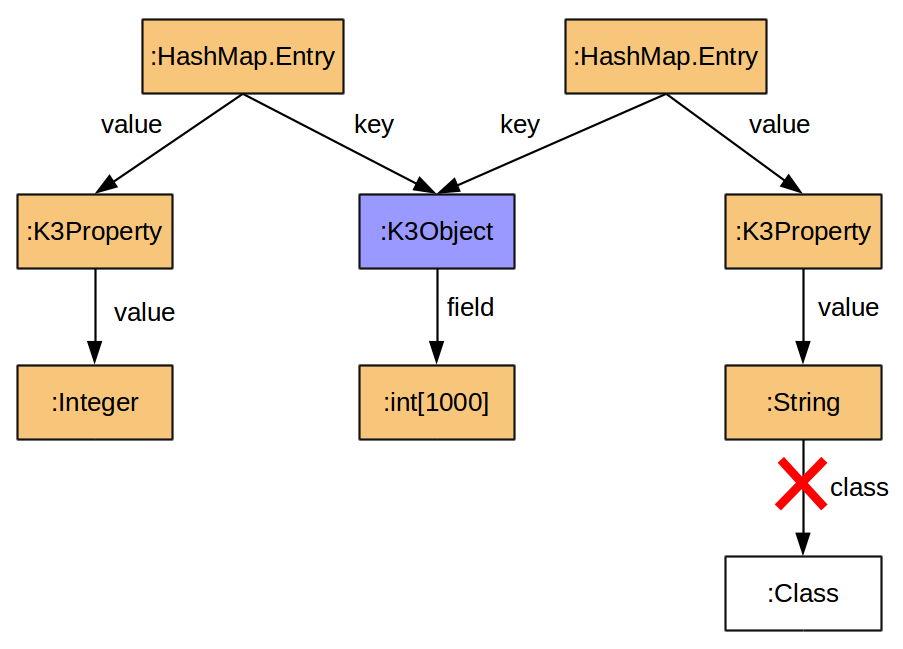
\includegraphics[scale=0.4]{./chapter6/fig/k3objects.png}
\caption{Snapshot of memory with one K3 Object. The idea is to compute the memory used by the shaded objects.} \label{fig:dsl-k3-example}
\end{figure}

To define this profiler, a good understanding of the implementation of K3-Objects, and their aspects, is needed.
We define a factory where a list of \textit{K3Objects} is used to identify the structures (see line 1 in Listing~\ref{k3}).
Hence, there will be as many structures as instances of class \textit{K3Objects}.
In line 3, the initial members of each structure are defined; notice that the membership function is parametrized by a K3Object instance, namely `$e$'.
The recursive case is then similar to previous examples, the difference is that we don't count instances of Class; this is shown in Figure~\ref{fig:dsl-k3-example}).


\begin{lstlisting}[escapeinside={(*}{*)},
caption=Computing the consumption of each K3-Al Object along with its aspects., 
label=k3,
%float=!h, 
language=DSL2]
create structure foreach e:objects(*{.filter}*)([it|it is K3Object]) using
  constructor
    initialObjects = objects.filter([
				    o| ret (o is HashMap.Entry) and (o.key == e)
				   ]).add(e)
    size = 0
  // the second part can be more precisely written as reference_kind != class_ref
  membership (referrer in this_structure) and not (this is java.lang.Class);
  updates
    size = size + this.size
\end{lstlisting}